\documentclass[11pt,a4paper]{article}
\usepackage[margin=2.3cm]{geometry}
\usepackage{amsmath,amssymb,graphicx,booktabs,microtype}
\usepackage[colorlinks,linkcolor=blue,urlcolor=blue]{hyperref}
\newcommand{\R}{\mathbb{R}}
\newcommand{\bu}{\boldsymbol u}
\newcommand{\bv}{\boldsymbol v}
\newcommand{\bX}{\boldsymbol X}
\newcommand{\bn}{\boldsymbol n}
\newcommand{\bt}{\boldsymbol t}
\newcommand{\bc}{\boldsymbol c}
\newcommand{\Ptau}{\boldsymbol P}
\title{A Halloween ghost in NGSolve:\\ nonlinear HHJ shell with frictional contact}
\author{Joachim Sch\"oberl}
\date{NGSolve Technical Note 2026-04\quad\textbullet\quad October 2026}

\begin{document}
\maketitle

\begin{figure}[h]
  \centering
  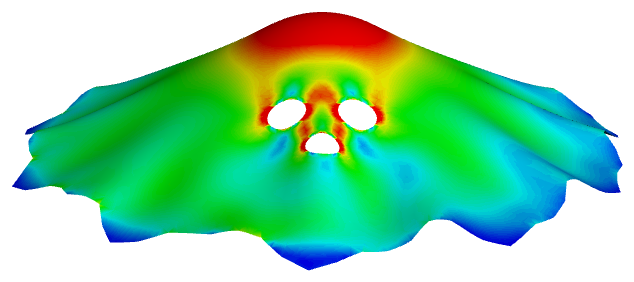
\includegraphics[width=0.418\textwidth]{w0022.png}\hfill
  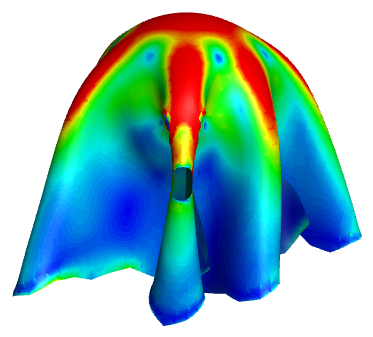
\includegraphics[width=0.246\textwidth]{w0050.png}\hfill
  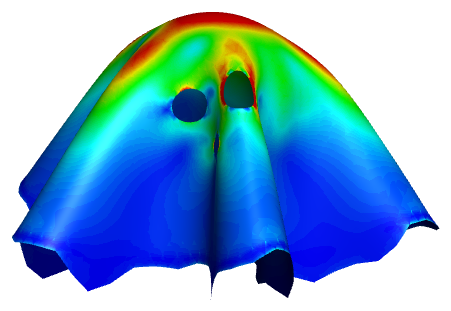
\includegraphics[width=0.297\textwidth]{w0330.png}
  \caption{A sheet with eye and mouth holes falls onto an invisible sphere, then is dragged
  around by it ($t = 0.44,\ 1,\ 6.6$). Rendered with the NGSolve webgui (curved order-2 elements); colour: norm of the Regge-interpolated membrane strain $|E_r|$, range $[0, 0.085]$.}
\end{figure}

\section{Setting}
A flat circular sheet $S \subset \R^3$ of radius $1.2$, with a slightly ragged hem
$r(\theta) = 1.2\,(1 + 0.04\sin 11\theta + 0.025\sin(23\theta+1))$ and three elliptic
holes (eyes and mouth), starts at rest at height $z_0 = 0.6$ above a sphere (``head'') of
radius $R_h = 0.35$. The head is at rest until $t = 2.5$, then follows a smoothly ramped
path
\[
  \bc(t) = \bigl(1-e^{-s/0.7}\bigr)\bigl(0.55\sin 1.3s,\ 0.15\sin 0.9s,\ 0.45\sin^2 0.7s\bigr),
  \qquad s = t - 2.5 .
\]
The sheet is a surface mesh in 3D with 3804 triangles ($h = 0.05$). The unknown is the
displacement $\bu : S \to \R^3$; the deformed position is $\bX + \bu$.

\section{Shell model}

\paragraph{Kinematics.}
With the unit normal $\bn$ of the reference surface and the tangential projection
$\Ptau = I - \bn\otimes\bn$, the surface deformation gradient and Green strain are
\[
  F = \nabla_\tau \bu + \Ptau, \qquad E = \tfrac12 (F^T F - \Ptau),
\]
and the deformed normal is $\bn_{\mathrm{def}} = \operatorname{cof}(F)\bn / |\operatorname{cof}(F)\bn|$.

\paragraph{Membrane.}
To avoid membrane locking, $E$ is interpolated into lowest-order Regge elements
($H(\mathrm{curl\,curl})$, order 1), $E_r = \mathcal I^{\mathrm{Regge}} E$. The membrane energy
is compressible neo-Hooke,
\[
  W_{\mathrm{mem}} = \frac{\mu}{2}(\operatorname{tr} C - 2) - \mu \ln J + \frac{\lambda}{2} (\ln J)^2,
  \qquad C = 2E_r + \Ptau,\quad J^2 = \det(C + \bn\otimes\bn),
\]
with $\mu = 500$, $\lambda = 200$ (per unit area). St.\,Venant--Kirchhoff was used first, but it
loses convexity for stretches below $1/\sqrt3$, which happens at the tips of the holes when
the sheet is compressed; Newton then stalled.

\paragraph{Bending: hybridized Hellan--Herrmann--Johnson.}
We use the nonlinear HHJ shell element of Neunteufel and Sch\"oberl. The bending moment
$\sigma$ is an independent unknown in $H(\mathrm{div\,div})$ on the surface. The bending
part of the Lagrangian is
\[
  \sum_{T} \int_T \Bigl( -\tfrac12\, \mathcal M^{-1}\sigma : \sigma + \sigma : H_\nu(\bu) \Bigr)
  + \sum_T \int_{\partial T} \Bigl( \sphericalangle(\boldsymbol\mu_{\mathrm{def}}, \bar{\boldsymbol\mu}) - \tfrac{\pi}{2}
     + \alpha\cdot\boldsymbol\mu \Bigr)\, \sigma_{\mu\mu},
\]
where
\begin{itemize}
  \item $H_\nu(\bu) = \sum_i (\nabla^2 \bu_i)\,(\bn_{\mathrm{def}})_i$ is the Hessian of the
        deformation contracted with the deformed normal;
  \item $\boldsymbol\mu$ is the outer conormal of the element edge; $\boldsymbol\mu_{\mathrm{def}}
        = \bn_{\mathrm{def}} \times \bt_{\mathrm{def}}$ is the deformed one;
  \item $\bar{\boldsymbol\mu}$ is an averaged normal on each edge (a vector facet field,
        order 2), updated once per time step from the current deformed normal and projected
        orthogonal to the deformed edge tangent. The edge angle measures the kink of the
        deformed surface across edges; $\pi/2$ is its value for the flat reference sheet;
  \item the material law is
        $\mathcal M^{-1}\sigma:\sigma = \frac{1+\nu}{D}\bigl(|\sigma|^2 - \frac{\nu}{1+\nu}(\operatorname{tr}\sigma)^2\bigr)$,
        i.e.\ the Kirchhoff plate law with $D = Et^3/12$; here $D = 0.05$, $\nu = 0.3$.
\end{itemize}

\paragraph{Hybridization.}
$\sigma$ is taken \emph{discontinuous} (\texttt{HDivDivSurface} with \texttt{discontinuous=True}),
and the normal-normal continuity of $\sigma$ is restored by the Lagrange multiplier
$\alpha$ in \texttt{NormalFacetSurface} (order 1), which plays the role of the rotation
across edges. On the free boundary (hem and hole rims) $\alpha$ has no boundary
condition, which gives $\sigma_{\mu\mu} = 0$ weakly. Since $\sigma$ is now element-local, it is
eliminated by static condensation; the condensed system in $(\bu, \alpha)$ is symmetric
positive definite and is solved with a sparse Cholesky factorization. (The non-hybridized
mixed form is a saddle point problem and needed a general LU.)

Sanity check: a cantilever strip under small load gives a tip deflection of
$-0.024988$ vs.\ $-qL^4/(8D) = -0.025$.

\section{Contact, damping and loads}
\begin{itemize}
  \item \textbf{Contact} with the analytic sphere by a penalty on the signed distance:
        $\frac{k_c}{2} [R_h - |\bX + \bu - \bc(t)|]_+^2$, $k_c = 2\cdot 10^4$.
  \item \textbf{Contact friction} as viscous drag relative to the head velocity $\bv_h$,
        active where the sheet was within $0.02$ of the head in the previous step
        ($\chi^n \in \{0,1\}$), $c_f = 200$.
  \item \textbf{Air drag} everywhere, $c_a = 3$. Without it the heavy hem swings under the
        head, folds through itself and an element inverts ($\ln J$ undefined).
  \item \textbf{Gravity} $g = 9.81$; areal density $\rho = 1$, and $\rho = 2$ in the hem
        ring $r > 1$.
\end{itemize}

\section{Time stepping}
Implicit Euler written as an incremental energy: in each step we find the stationary point
of
\[
\begin{aligned}
  \Pi^{n+1}(\bu,\sigma,\alpha) = \int_S \Bigl[\, & \frac{\rho}{2\Delta t^2}\,|\bu - \bu^n - \Delta t\, \bv^n|^2
  + W_{\mathrm{mem}}(\bu) + \rho g\, u_z
  + \frac{k_c}{2} [R_h - |\bX + \bu - \bc^{n+1}|]_+^2 \\
  & + \frac{c_f \chi^n + c_a}{2\Delta t}\, |\bu - \bu^n - \Delta t\, \bv_h|^2 \Bigr]
  + \text{(HHJ bending terms)},
\end{aligned}
\]
then set $\bv^{n+1} = (\bu^{n+1} - \bu^n)/\Delta t$. The step is $\Delta t = 0.01$, 800 steps
for $t \in [0, 8]$. Each step uses Newton on the condensed system, starting from the
predictor $\bu^n + \Delta t\,\bv^n$. A Newton update is halved while the residual is not
finite (inverted element); a failed step would be retried with $\Delta t/2$, recursively
down to $\Delta t/16$. In the final run no step needed this: 2--6 Newton iterations
per step.

\paragraph{Discretization summary.}
\begin{center}
\begin{tabular}{ll}
\toprule
displacement $\bu$ & \texttt{VectorH1}, order 2 \\
moment $\sigma$ & \texttt{HDivDivSurface}, order 1, discontinuous (condensed) \\
multiplier $\alpha$ & \texttt{NormalFacetSurface}, order 1 \\
membrane strain & Regge interpolation, \texttt{HCurlCurl} order 1 \\
averaged normal $\bar{\boldsymbol\mu}$ & \texttt{VectorFacetSurface}, order 2 \\
unknowns & 69\,426 total, 35\,190 after condensation \\
linear solver & sparse Cholesky \\
\bottomrule
\end{tabular}
\end{center}

\section{Implementation notes}
\begin{itemize}
  \item Each energy term is its own \texttt{Variation}; a single summed \texttt{Variation}
        linearized about $20\times$ slower. The membrane, bending and edge terms are
        \texttt{Compile()}d.
  \item Assembling the linearization takes about 0.7\,s per Newton iteration and dominates;
        the Cholesky factorization takes about 0.05\,s.
  \item The total run is roughly 30--80 minutes on an Apple M4 (depending on threads).
  \item Visualization: the order-2 displacement is drawn with the NGSolve webgui as curved
        Bernstein triangles; frames are captured with headless Chrome and encoded to H.264.
\end{itemize}

\paragraph{Reference.}
M.~Neunteufel, J.~Sch\"oberl, \emph{The Hellan--Herrmann--Johnson method for nonlinear
shells}, Computers \& Structures 225 (2019); M.~Neunteufel, J.~Sch\"oberl, \emph{Avoiding
membrane locking with Regge interpolation}, CMAME 373 (2021); see also the ESI minicourse
\url{https://jschoeberl.github.io/ESI-Elasticity-Geometry-NGSolve/ESI-minicourse.html}.

\end{document}
